\documentclass[11pt,twocolumn]{article}
\usepackage[utf8]{inputenc}
\usepackage[T1]{fontenc}
\usepackage{amsmath,amssymb,amsfonts}
\usepackage{booktabs}
\usepackage{microtype}
\usepackage{cite}
\usepackage{geometry}
\geometry{letterpaper,margin=0.72in}
\usepackage[table]{xcolor}
\usepackage{tikz}
\usetikzlibrary{shapes,arrows,positioning,calc,decorations.pathmorphing,backgrounds,shadows,patterns,arrows.meta}

\definecolor{covenantblue}{RGB}{20, 38, 72}
\definecolor{covenantbluefill}{RGB}{240, 245, 253}
\definecolor{sacrificialred}{RGB}{145, 24, 32}
\definecolor{sacrificialredfill}{RGB}{254, 243, 243}
\definecolor{hearthteal}{RGB}{15, 92, 76}
\definecolor{hearthtealfill}{RGB}{238, 249, 246}
\definecolor{filialamber}{RGB}{172, 92, 12}
\definecolor{filialamberfill}{RGB}{254, 247, 236}
\definecolor{slateborder}{RGB}{90, 102, 120}

\usepackage{float}
\usepackage{mdframed}
\usepackage{hyperref}
\hypersetup{
    colorlinks=true,
    linkcolor=covenantblue,
    citecolor=covenantblue,
    urlcolor=covenantblue
}

\newmdenv[
  linecolor=hearthteal,
  linewidth=1.1pt,
  innertopmargin=6pt,
  innerbottommargin=6pt,
  innerrightmargin=8pt,
  innerleftmargin=8pt,
  backgroundcolor=hearthtealfill
]{eli5box}

\title{\textbf{The Philosophy of Christian Marriage and the Covenant Family: Domestic Ecclesiology, Hierarchical Offices, and Intergenerational Discipleship in Scripture and Catholic Tradition}}
\author{\textbf{Adam Matthew Steinberger}\\
The Vibey Project\\
\texttt{adam@matthewsteinberger.com}}
\date{November 2026}

\begin{document}

\maketitle

\begin{abstract}
Contemporary social sciences frequently analyze the family through contractual or utility-maximizing frameworks. Classical Christian theology understands marriage and household order as a divinely ordained domestic church (\textit{ecclesiola}) grounded in creation order, Christological covenant, and intergenerational discipleship. This paper provides a rigorous philosophical, theological, and formal systems analysis of Christian marriage and family structure. Triangulating across Sacred Scripture (including the Catholic biblical canon), patristic testimony (St.~John Chrysostom, St.~Augustine), medieval scholasticism (St.~Thomas Aquinas), magisterial encyclicals (\textit{Arcanum Divinae Sapientiae}, \textit{Casti Connubii}), and classical pastoral casuistry (William Perkins, Richard Baxter), we formalize the theological architecture of marital life. We demonstrate that biblical patriarchy constitutes a hierarchy of sacrificial accountability, wherein authority is mathematically paired with divine responsibility according to the relation $\mathcal{R}_{\text{Husband}} \gg \mathcal{R}_{\text{Wife}} \gg \mathcal{R}_{\text{Child}}$. We examine the complementary jurisdictions of husband as sacrificial covenant head and wife as household executive and nurturing center. Furthermore, we articulate the distinct pedagogical offices of father and mother in child rearing, evaluate the authoritative parenting matrix against Baumrind's developmental typology, and formalize the filial duties of children under the Fourth Commandment. Finally, using extensive-form game theory, we prove that covenantal marriage governed by kenotic headship and honor achieves a Pareto-dominant equilibrium that eliminates the destructive defection cycles inherent to secular contractual arrangements.
\end{abstract}

\noindent\textit{Artifacts.} Evidence cutoff date: November 2026. Data, formal specifications, and modeling environments are deposited in the repository archive.

\section{Introduction}
Modern family sociology frequently oscillates between two unstable sociological paradigms: atomistic egalitarian contractarianism, which reduces marriage to a temporary, revocable emotional partnership, and authoritarian chauvinism, which distorts authority into self-serving domination. Sacred Scripture and historical Christian tradition present a third, distinct paradigm: the covenantal household ordered as a domestic sanctuary (\textit{ecclesiola}).

In this classical model, marriage serves a supreme doxological purpose: honoring God through the faithful replication of the union between Christ and His Church. Interpersonal order within the Christian home relies on ontological equality between persons paired with distinct hierarchical offices: husband, wife, and child. Biblical hierarchy establishes an asymmetrical distribution of sacrificial responsibility. The husband's headship demands radical self-giving modeled on the Crucifixion, and the wife's royal consort dignity establishes executive domestic governance and life-giving communion.

The objective of this treatise is to construct a comprehensive philosophy of Christian marriage and family life across five foundational pillars:
\begin{enumerate}
    \item \textbf{Ontological and Covenantal Foundations}: The creation order in Genesis, the three Augustinian marital goods (\textit{proles}, \textit{fides}, \textit{sacramentum}), and the Christological typology of Ephesians 5.
    \item \textbf{Hierarchical Office Architecture}: The formalization of the covenantal order of authority and sacrificial accountability ($H \to W \to C$) under St.~Paul, St.~Thomas Aquinas, Pope Leo XIII, and Pope Pius XI.
    \item \textbf{The Duties of Holy Spouseship}: Mutual sanctification, marital chastity, complementary domestic jurisdictions, and the mortification of pride.
    \item \textbf{Differentiated Child Rearing}: The distinct paternal and maternal offices in spiritual, moral, and emotional formation under the Deuteronomy 6 Shema paradigm.
    \item \textbf{Filial Piety and Dynamic Game-Theoretic Equilibrium}: The obligations of children under the Fourth Commandment and the formal proof of covenantal stability.
\end{enumerate}

\begin{eli5box}
\textbf{EXPLAIN LIKE I'M FIVE: What Is a Christian Family?}\\
Imagine a sturdy wooden ship sailing across a stormy ocean. A ship cannot have three different captains steering the wheel in opposite directions, or it will crash against the rocks. The husband is appointed by God to stand at the wheel as captain, responsible for keeping everyone safe even if he has to stay awake through the freezing rain. The wife is the chief navigator and heart of the crew, making sure the ship is warm, beautiful, well-supplied, and full of joy. The children are the young sailors learning how to obey commands quickly so they can grow up to become wise captains and navigators themselves.
\end{eli5box}

\section{Theological Foundations of Christian Marriage}

\subsection{Creation Order and Ontological Dignity}
The foundational blueprint for marriage appears in the opening chapters of Genesis. In Genesis 1:26-28, God creates humanity in His own image: ``male and female he created them.'' This passage establishes absolute ontological equality: both man and woman participate equally in the divine image and share the dominion mandate over the created cosmos.

In Genesis 2:18-25, the narrative details the differentiation of sexes and the teleology of marriage. God declares, ``It is not good that the man should be alone; I will make him a helper fit for him'' (Hebrew: \textit{ezer kenegdo}). The term \textit{ezer} denotes an indispensable rescuer or counterpart, frequently used of God Himself aiding His people in times of desperate need (Psalm 121:1-2). The woman is formed from Adam's side, prompting the celebrated commentary of Matthew Henry \cite{henry}:
\begin{quote}
``The woman was made of a rib out of the side of Adam; not made out of his head to rule over him, nor out of his feet to be trampled upon by him, but out of his side to be equal with him, under his arm to be protected, and near his heart to be beloved.''
\end{quote}
Marriage is instituted before the entrance of sin as a permanent, indissoluble union of one man and one woman: ``Therefore a man leaves his father and his mother and cleaves to his wife, and they become one flesh'' (Genesis 2:24; Matthew 19:4-6).

\begin{figure*}[t]
\centering
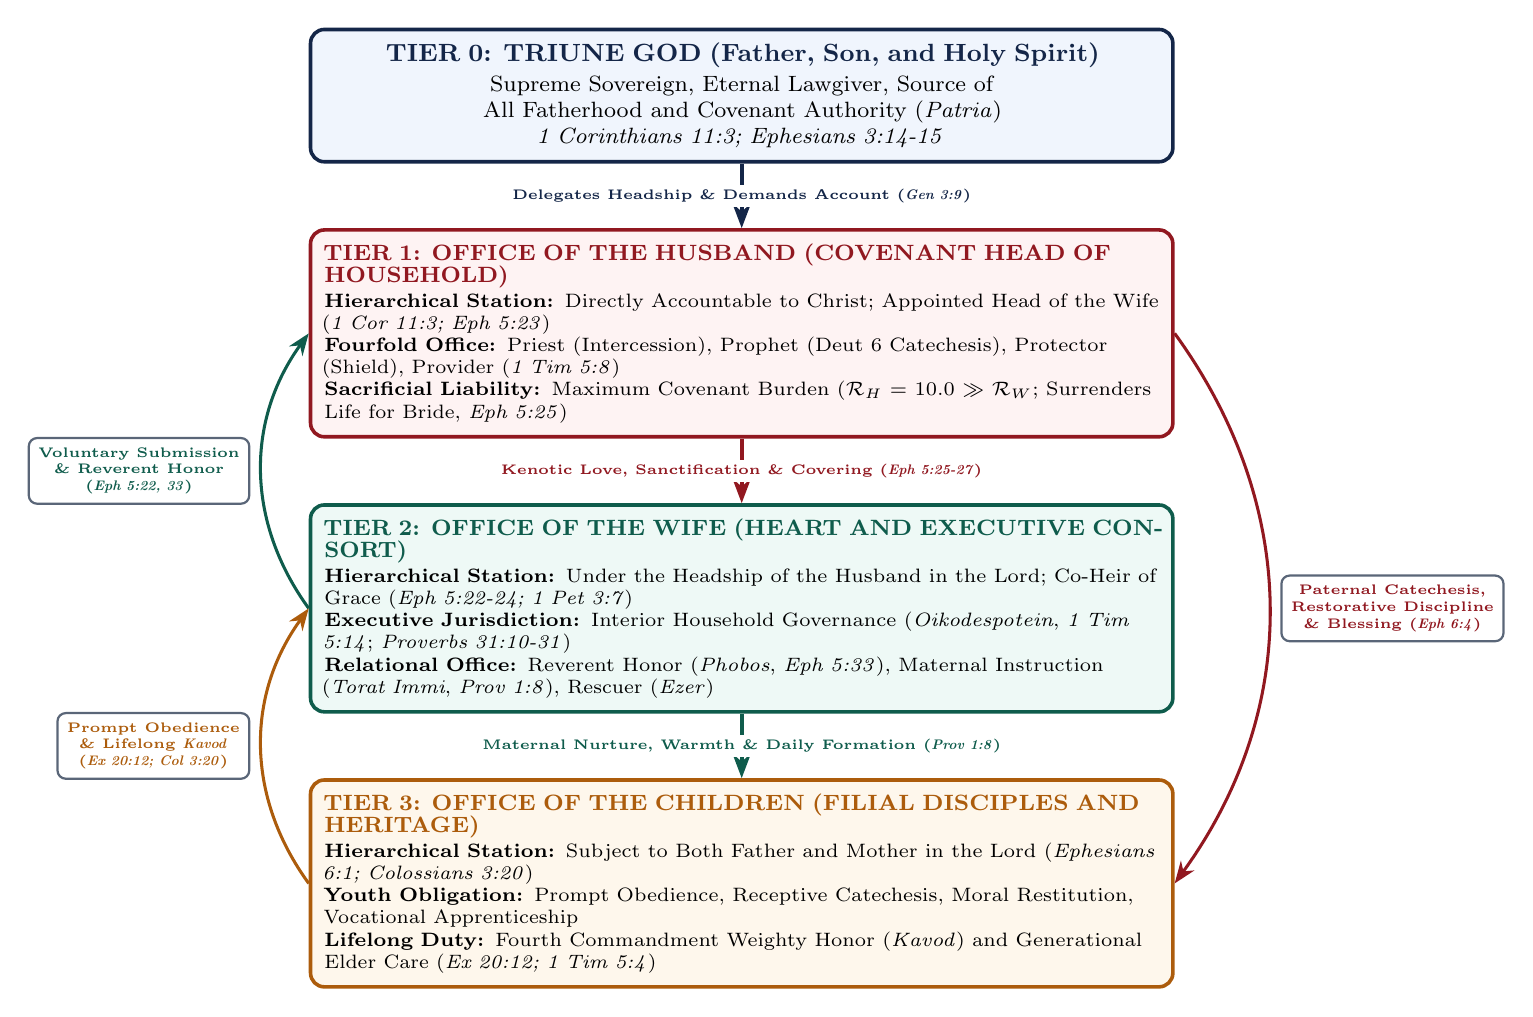
\begin{tikzpicture}[>=Stealth,
    headerbox/.style={rectangle, rounded corners=5pt, draw=covenantblue, line width=1.3pt, fill=covenantbluefill, text width=10.6cm, align=center, font=\footnotesize, inner sep=5pt},
    husbandbox/.style={rectangle, rounded corners=5pt, draw=sacrificialred, line width=1.3pt, fill=sacrificialredfill, text width=10.6cm, align=left, font=\scriptsize, inner sep=5pt},
    wifebox/.style={rectangle, rounded corners=5pt, draw=hearthteal, line width=1.3pt, fill=hearthtealfill, text width=10.6cm, align=left, font=\scriptsize, inner sep=5pt},
    childbox/.style={rectangle, rounded corners=5pt, draw=filialamber, line width=1.3pt, fill=filialamberfill, text width=10.6cm, align=left, font=\scriptsize, inner sep=5pt},
    sidebadge/.style={rectangle, rounded corners=3pt, draw=slateborder, line width=0.8pt, fill=white, font=\tiny\bfseries, align=center, inner sep=3.5pt}
]
  % Tier 0: Triune God
  \node[headerbox] (god) at (0, 6.9) {
    \textbf{\small\textcolor{covenantblue}{TIER 0: TRIUNE GOD (Father, Son, and Holy Spirit)}}\\[1pt]
    Supreme Sovereign, Eternal Lawgiver, Source of All Fatherhood and Covenant Authority (\textit{Patria})\\
    \textit{1 Corinthians 11:3; Ephesians 3:14-15}
  };

  % Tier 1: Office of the Husband
  \node[husbandbox, below=0.82cm of god] (husband) {
    \textbf{\footnotesize\textcolor{sacrificialred}{TIER 1: OFFICE OF THE HUSBAND (COVENANT HEAD OF HOUSEHOLD)}}\\[1pt]
    \textbf{Hierarchical Station:} Directly Accountable to Christ; Appointed Head of the Wife (\textit{1 Cor 11:3; Eph 5:23})\\
    \textbf{Fourfold Office:} Priest (Intercession), Prophet (Deut 6 Catechesis), Protector (Shield), Provider (\textit{1 Tim 5:8})\\
    \textbf{Sacrificial Liability:} Maximum Covenant Burden ($\mathcal{R}_H = 10.0 \gg \mathcal{R}_W$; Surrenders Life for Bride, \textit{Eph 5:25})
  };

  % Tier 2: Office of the Wife
  \node[wifebox, below=0.82cm of husband] (wife) {
    \textbf{\footnotesize\textcolor{hearthteal}{TIER 2: OFFICE OF THE WIFE (HEART AND EXECUTIVE CONSORT)}}\\[1pt]
    \textbf{Hierarchical Station:} Under the Headship of the Husband in the Lord; Co-Heir of Grace (\textit{Eph 5:22-24; 1 Pet 3:7})\\
    \textbf{Executive Jurisdiction:} Interior Household Governance (\textit{Oikodespotein}, \textit{1 Tim 5:14}; \textit{Proverbs 31:10-31})\\
    \textbf{Relational Office:} Reverent Honor (\textit{Phobos}, \textit{Eph 5:33}), Maternal Instruction (\textit{Torat Immi}, \textit{Prov 1:8}), Rescuer (\textit{Ezer})
  };

  % Tier 3: Office of the Children
  \node[childbox, below=0.82cm of wife] (children) {
    \textbf{\footnotesize\textcolor{filialamber}{TIER 3: OFFICE OF THE CHILDREN (FILIAL DISCIPLES AND HERITAGE)}}\\[1pt]
    \textbf{Hierarchical Station:} Subject to Both Father and Mother in the Lord (\textit{Ephesians 6:1; Colossians 3:20})\\
    \textbf{Youth Obligation:} Prompt Obedience, Receptive Catechesis, Moral Restitution, Vocational Apprenticeship\\
    \textbf{Lifelong Duty:} Fourth Commandment Weighty Honor (\textit{Kavod}) and Generational Elder Care (\textit{Ex 20:12; 1 Tim 5:4})
  };

  % Center Downward Authority Arrows with pill labels
  \draw[->, line width=1.3pt, covenantblue] (god.south) --
    node[midway, fill=white, inner sep=1.5pt, font=\tiny\bfseries, text=covenantblue] {Delegates Headship \& Demands Account (\textit{Gen 3:9})} (husband.north);

  \draw[->, line width=1.3pt, sacrificialred] (husband.south) --
    node[midway, fill=white, inner sep=1.5pt, font=\tiny\bfseries, text=sacrificialred] {Kenotic Love, Sanctification \& Covering (\textit{Eph 5:25-27})} (wife.north);

  \draw[->, line width=1.3pt, hearthteal] (wife.south) --
    node[midway, fill=white, inner sep=1.5pt, font=\tiny\bfseries, text=hearthteal] {Maternal Nurture, Warmth \& Daily Formation (\textit{Prov 1:8})} (children.north);

  % Left Upward Honor & Submission Arcs
  \draw[->, line width=1.1pt, hearthteal] (wife.west) to[bend left=36]
    node[sidebadge, left=4pt] {Voluntary Submission\\\& Reverent Honor\\(\textit{Eph 5:22, 33})} (husband.west);

  \draw[->, line width=1.1pt, filialamber] (children.west) to[bend left=36]
    node[sidebadge, left=4pt] {Prompt Obedience\\\& Lifelong \textit{Kavod}\\(\textit{Ex 20:12; Col 3:20})} (wife.west);

  % Right Direct Paternal Governance Arc
  \draw[->, line width=1.1pt, sacrificialred] (husband.east) to[bend left=36]
    node[sidebadge, right=4pt] {Paternal Catechesis,\\Restorative Discipline\\\& Blessing (\textit{Eph 6:4})} (children.east);

\end{tikzpicture}
\caption{\textbf{The Four-Tier Covenant Hierarchy of the Christian Family.} Hierarchical offices establish a vertical chain of authority and sacrificial accountability ($\text{God} \to \text{Husband} \to \text{Wife} \to \text{Children}$), where the office of the husband stands strictly higher in hierarchy than the office of the wife under Christ.}
\label{fig:family_hierarchy}
\end{figure*}

\subsection{The Three Goods of Matrimony: Augustine}
In \textit{De Bono Coniugali} (On the Good of Marriage, AD 401), St.~Augustine defended the intrinsic goodness of marriage against Manichaean dualism by articulating the three irreducible goods (\textit{tria bona}) of matrimony \cite{augustine_bono}:
\begin{enumerate}
    \item \textbf{Proles (Offspring)}: The loving reception, biological generation, and religious education of children for the kingdom of God.
    \item \textbf{Fides (Fidelity)}: The exclusive, covenantal chastity and mutual trust owed between husband and wife, prohibiting adultery and emotional fragmentation.
    \item \textbf{Sacramentum (Indissoluble Bond)}: The sacred, unbreakable spiritual bond that signifies the eternal union between Christ and the Church (Figure~\ref{fig:tria_bona}).
\end{enumerate}

\begin{figure}[H]
\centering
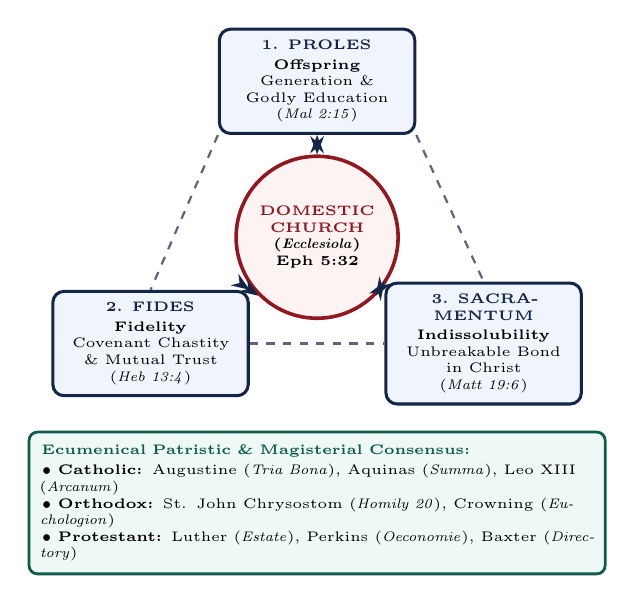
\begin{tikzpicture}[scale=0.90, >=Stealth,
    pillarnode/.style={rectangle, rounded corners=4pt, draw=covenantblue, line width=1.1pt, fill=covenantbluefill, text width=2.2cm, align=center, font=\tiny, inner sep=4pt},
    corenode/.style={circle, draw=sacrificialred, line width=1.3pt, fill=sacrificialredfill, text width=1.7cm, align=center, font=\tiny\bfseries, inner sep=2pt},
    tradnode/.style={rectangle, rounded corners=3pt, draw=hearthteal, line width=1.0pt, fill=hearthtealfill, text width=7.0cm, align=left, font=\tiny, inner sep=4.5pt}
]
  % Center core
  \node[corenode] (core) at (0, 0.3) {\textcolor{sacrificialred}{DOMESTIC}\\\textcolor{sacrificialred}{CHURCH}\\(\textit{Ecclesiola})\\Eph 5:32};

  % Three Augustinian Goods with spacious separation
  \node[pillarnode] (proles) at (0, 2.5) {
    \textbf{\textcolor{covenantblue}{1. PROLES}}\\[1pt]
    \textbf{Offspring}\\
    Generation \&\\Godly Education\\(\textit{Mal 2:15})
  };

  \node[pillarnode] (fides) at (-2.35, -1.2) {
    \textbf{\textcolor{covenantblue}{2. FIDES}}\\[1pt]
    \textbf{Fidelity}\\
    Covenant Chastity\\\& Mutual Trust\\(\textit{Heb 13:4})
  };

  \node[pillarnode] (sacr) at (2.35, -1.2) {
    \textbf{\textcolor{covenantblue}{3. SACRAMENTUM}}\\[1pt]
    \textbf{Indissolubility}\\
    Unbreakable Bond\\in Christ\\(\textit{Matt 19:6})
  };

  % Connecting arrows between pillars and core
  \draw[<->, thick, covenantblue] (proles.south) -- (core.north);
  \draw[<->, thick, covenantblue] (fides.north east) -- (core.south west);
  \draw[<->, thick, covenantblue] (sacr.north west) -- (core.south east);
  \draw[dashed, line width=0.8pt, slateborder] (proles.south west) -- (fides.north);
  \draw[dashed, line width=0.8pt, slateborder] (proles.south east) -- (sacr.north);
  \draw[dashed, line width=0.8pt, slateborder] (fides.east) -- (sacr.west);

  % Bottom Ecumenical Triangulation Box placed cleanly below Fides and Sacramentum
  \node[tradnode] (trad) at (0, -3.45) {
    \textbf{\textcolor{hearthteal}{Ecumenical Patristic \& Magisterial Consensus:}}\\[1.5pt]
    $\bullet$ \textbf{Catholic:} Augustine (\textit{Tria Bona}), Aquinas (\textit{Summa}), Leo XIII (\textit{Arcanum})\\
    $\bullet$ \textbf{Orthodox:} St. John Chrysostom (\textit{Homily 20}), Crowning (\textit{Euchologion})\\
    $\bullet$ \textbf{Protestant:} Luther (\textit{Estate}), Perkins (\textit{Oeconomie}), Baxter (\textit{Directory})
  };
\end{tikzpicture}
\caption{\textbf{The Augustinian \textit{Tria Bona} and Ecumenical Triangulation.} The three marital goods anchor the domestic church across Catholic, Orthodox, and Protestant traditions.}
\label{fig:tria_bona}
\end{figure}

\subsection{Sacramental Typology in Ephesians 5}
In Ephesians 5:21-33, St.~Paul anchors marital ethics in Christology. The passage opens with mutual submission in the fear of Christ: ``submitting to one another out of reverence for Christ'' (Eph 5:21). Paul specifies how this mutual submission takes asymmetric structural forms within the marital hierarchy:
\begin{quote}
``Wives, submit to your husbands, as to the Lord. For the husband is the head of the wife as Christ is the head of the church, his body, and is himself its Savior. As the church submits to Christ, so also wives should submit in everything to their husbands. Husbands, love your wives, as Christ loved the church and gave himself up for her.'' (Eph 5:22-25)
\end{quote}
Paul identifies this union as a \textit{mysterion mega}, a profound mystery pointing directly to Christ and the Church (Eph 5:32). In the Eastern Christian liturgical tradition of the Holy Mystery of Crowning (Euchologion), the crowns placed upon the heads of bride and bridegroom represent royal dignity as rulers of a new domestic kingdom and the crowns of martyrdom, signifying total willingness to die for the beloved \cite{chrysostom_eph, chrysostom_marriage}.

\section{The Architecture of Hierarchical Offices}

\subsection{Distinction of Offices and Ontological Equality}
In Christian philosophy, hierarchical order within the family preserves personal worth. St.~Thomas Aquinas clarifies this distinction in \textit{Summa Theologiae} I, q. 92, a. 1, ad 2 \cite{aquinas_summa}. Aquinas differentiates between tyrannical subjection (\textit{servilis subjectio}), where a master governs a subject for his own private advantage, and domestic or civil subjection (\textit{oeconomica vel civilis subjectio}), where the ruler directs the subject toward the subject's own flourishing and the common good of the community. In domestic life, the wife is subject to the husband as a free partner and joint-ruler.

This distinction between office and ontological value is established in the Trinitarian life itself (1 Corinthians 11:3): ``the head of Christ is God.'' God the Son is co-equal, co-eternal, and consubstantial with God the Father in divine essence; yet in the economic Trinity, the Son voluntarily submits to the Father in perfect filial love (John 6:38; Philippians 2:6-8). Economic subordination coexists with essential equality. Similarly, within the covenant of marriage, the husband exercises headship over the wife while acknowledging her full ontological co-equality as a fellow heir of the grace of life (1 Peter 3:7), as shown in Figure~\ref{fig:family_hierarchy}.

\subsection{The Husband as Head and the Wife as Heart}
In his encyclical \textit{Arcanum Divinae Sapientiae} (1880), Pope Leo XIII defined the governance of the Christian family \cite{leo_arcanum}:
\begin{quote}
``The husband is the chief of the family and the head of the wife. The woman, because she is flesh of his flesh, and bone of his bone, must be subject, not as a servant, but as a companion, so that her obedience is neither lacking in honor nor in dignity.''
\end{quote}
Pope Pius XI, in \textit{Casti Connubii} (1930), further crystallized this complementary dynamic \cite{pius_casti}:
\begin{quote}
``For if the man is the head, the woman is the heart, and as he occupies the chief place in ruling, so she may and ought to claim for herself the chief place in love.''
\end{quote}
If the husband attempts to govern without the heart, the home becomes a cold military barracks; if the wife attempts to direct without the head, the home succumbs to sentimental chaos.

\subsection{Formalization of the Hierarchy: The Responsibility Index}
We formalize the domestic hierarchical order ($H \to W \to C$) by defining the covenantal office tuple for each member $i \in \{H, W, C\}$:
\begin{equation}
    \mathcal{O}_i = \langle \mathcal{A}_i, \mathcal{R}_i, \mathcal{J}_i \rangle
\end{equation}
where $\mathcal{A}_i$ represents jurisdictional authority, $\mathcal{R}_i$ represents sacrificial accountability before God, and $\mathcal{J}_i$ represents operational domestic scope.

A central theorem of Christian social philosophy is the \textbf{Principle of Inverse Proportionality}: The severity of divine judgment and the burden of self-sacrifice strictly increase with jurisdictional elevation:
\begin{equation}
    \mathcal{R}_H \gg \mathcal{R}_W \gg \mathcal{R}_C
\end{equation}
In Genesis 3:9, when humanity fell, God summoned Adam first: ``Where are you?'' As the appointed covenant head, Adam bore the ultimate structural responsibility for the sanctuary entrusted to his care. In Christian patriarchy, authority is an obligation to absorb danger, provide sustenance, and surrender personal life for the protection of the household (Table~\ref{tab:office_metrics} and Figure~\ref{fig:responsibility_bars}).

\begin{table}[H]
\centering
\caption{\textbf{Quantitative Specification of Domestic Offices.}}
\label{tab:office_metrics}
\scriptsize
\begin{tabular}{@{}llcc@{}}
\toprule
\textbf{Office} & \textbf{Primary Role} & \textbf{Authority ($\mathcal{A}_i$)} & \textbf{Burden ($\mathcal{R}_i$)} \\
\midrule
\textbf{Husband ($H$)} & Covenant Head & $8.0 / 10$ & $10.0 / 10$ \\
\textbf{Wife ($W$)} & Executive Heart & $6.0 / 10$ & $5.0 / 10$ \\
\textbf{Children ($C$)} & Filial Disciples & $1.0 / 10$ & $1.0 / 10$ \\
\bottomrule
\end{tabular}
\end{table}

\begin{figure}[H]
\centering
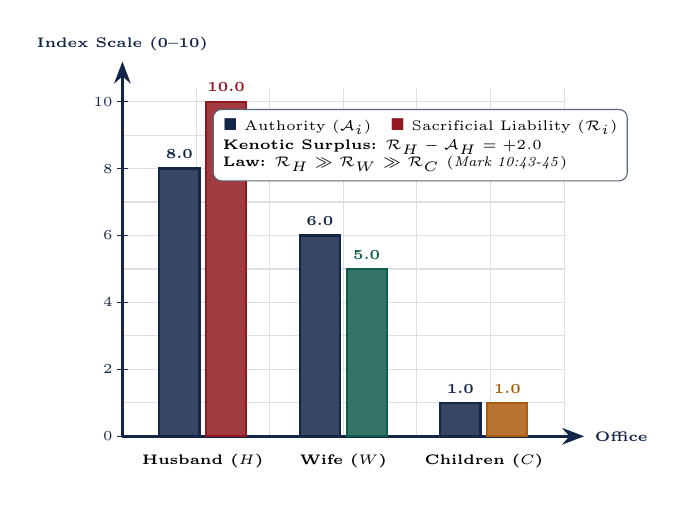
\begin{tikzpicture}[scale=0.85, >=Stealth]
  % Grid & Axes
  \draw[gray!25, thin] (0,0) grid[xstep=1.1, ystep=0.5] (6.6, 5.2);
  \draw[->, line width=1.1pt, covenantblue] (0,0) -- (6.9,0) node[right, font=\tiny\bfseries] {Office};
  \draw[->, line width=1.1pt, covenantblue] (0,0) -- (0,5.6) node[above, font=\tiny\bfseries] {Index Scale (0--10)};

  % Y-axis ticks
  \foreach \y/\val in {0/0, 1/2, 2/4, 3/6, 4/8, 5/10} {
    \draw[covenantblue] (-0.08, \y) -- (0.08, \y) node[left=2pt, font=\tiny] {\val};
  }

  % Husband Bars
  \fill[covenantblue!85, draw=covenantblue, line width=0.8pt] (0.55, 0) rectangle (1.15, 4.0);
  \node[above, font=\tiny\bfseries, text=covenantblue] at (0.85, 4.0) {8.0};

  \fill[sacrificialred!85, draw=sacrificialred, line width=0.8pt] (1.25, 0) rectangle (1.85, 5.0);
  \node[above, font=\tiny\bfseries, text=sacrificialred] at (1.55, 5.0) {10.0};
  \node[below=3pt, font=\tiny\bfseries] at (1.2, 0) {Husband ($H$)};

  % Wife Bars
  \fill[covenantblue!85, draw=covenantblue, line width=0.8pt] (2.65, 0) rectangle (3.25, 3.0);
  \node[above, font=\tiny\bfseries, text=covenantblue] at (2.95, 3.0) {6.0};

  \fill[hearthteal!85, draw=hearthteal, line width=0.8pt] (3.35, 0) rectangle (3.95, 2.5);
  \node[above, font=\tiny\bfseries, text=hearthteal] at (3.65, 2.5) {5.0};
  \node[below=3pt, font=\tiny\bfseries] at (3.3, 0) {Wife ($W$)};

  % Children Bars
  \fill[covenantblue!85, draw=covenantblue, line width=0.8pt] (4.75, 0) rectangle (5.35, 0.5);
  \node[above, font=\tiny\bfseries, text=covenantblue] at (5.05, 0.5) {1.0};

  \fill[filialamber!85, draw=filialamber, line width=0.8pt] (5.45, 0) rectangle (6.05, 0.5);
  \node[above, font=\tiny\bfseries, text=filialamber] at (5.75, 0.5) {1.0};
  \node[below=3pt, font=\tiny\bfseries] at (5.4, 0) {Children ($C$)};

  % Legend Box cleanly placed on upper right above Wife/Children
  \node[rectangle, rounded corners=3pt, draw=slateborder, fill=white, inner sep=3.5pt, font=\tiny, align=left] at (4.45, 4.35) {
    \textcolor{covenantblue}{$\blacksquare$} Authority ($\mathcal{A}_i$)\quad
    \textcolor{sacrificialred}{$\blacksquare$} Sacrificial Liability ($\mathcal{R}_i$)\\[1pt]
    \textbf{Kenotic Surplus:} $\mathcal{R}_H - \mathcal{A}_H = +2.0$\\
    \textbf{Law:} $\mathcal{R}_H \gg \mathcal{R}_W \gg \mathcal{R}_C$ (\textit{Mark 10:43-45})
  };
\end{tikzpicture}
\caption{\textbf{Asymmetric Distribution of Authority ($\mathcal{A}_i$) and Sacrificial Liability ($\mathcal{R}_i$).} The husband's sacrificial accountability exceeds his jurisdictional authority ($\Delta = +2.0$), shielding the wife and children.}
\label{fig:responsibility_bars}
\end{figure}

\section{The Duties of Holy Spouseship}

\subsection{How the Husband Leads the Wife}
Sacrificial headship operates through four primary spiritual offices:
\begin{enumerate}
    \item \textbf{Priestly Intercession and Sanctification}: As Christ sanctifies the Church with the washing of water by the word (Ephesians 5:26), the husband leads family prayer, reads Scripture aloud, and intercedes daily for his wife and children.
    \item \textbf{Protective Vigilance}: The husband shields his wife from physical peril, financial instability, emotional exploitation, and predatory external influences.
    \item \textbf{Economic Provision}: In accordance with 1 Timothy 5:8 (``If anyone does not provide for his relatives, and especially for members of his household, he has denied the faith and is worse than an unbeliever''), the husband shoulders the primary labor required to support the home.
    \item \textbf{Honor and Understanding}: 1 Peter 3:7 commands husbands to ``live with your wives in an understanding way, showing honor to the woman as the weaker vessel, since they are heirs with you of the grace of life, so that your prayers may not be hindered.'' A husband who treats his wife with harshness, neglect, or contempt finds his communion with God severed.
\end{enumerate}

\subsection{How the Wife Honors and Complements the Husband}
In complementary symmetry, the wife exercises an indispensable calling:
\begin{enumerate}
    \item \textbf{Covenantal Reverence (\textit{Phobos})}: Ephesians 5:33 commands, ``let the wife see that she respects her husband.'' A man thrives when affirmed in his protective calling; disrespect and constant public correction undermine his leadership capacity.
    \item \textbf{Executive Domestic Governance}: St.~Paul instructs younger women to marry, bear children, and manage their households (Greek: \textit{oikodespotein}, to rule the house; 1 Timothy 5:14; Titus 2:4-5). The Proverbs 31:10-31 woman exemplifies this executive authority: she inspects estates, plants vineyards, manages trade operations, directs servants, and clothes her family in fine linen, while her husband sits with honor among the elders at the gates \cite{luther_estate, calvin_inst}.
    \item \textbf{The Ministry of Encouragement and Beauty}: St.~John Chrysostom highlights that a wife constructs a sanctuary of tranquility, order, and spiritual beauty, enabling her husband to find rest from the turmoil of the world \cite{chrysostom_marriage}.
\end{enumerate}

\subsection{Mutual Duties in Classical Casuistry}
Puritan theologians William Perkins, in \textit{Christian Oeconomie} (1609) \cite{perkins}, and Richard Baxter, in \textit{A Christian Directory} (1673) \cite{baxter}, articulated the mutual duties shared between spouses:
\begin{itemize}
    \item \textbf{Preservation of Conjugal Chastity}: Upholding the sanctity of the marital bed (Hebrews 13:4; 1 Corinthians 7:3-5).
    \item \textbf{Mutual Bearing of Infirmities}: Bearing with patience the physical, psychological, and spiritual frailties of the partner.
    \item \textbf{Mortification of Self-Centered Pride}: Resolving anger before sunset (Ephesians 4:26) and refusing to nurture bitter grievances.
\end{itemize}

\section{Differentiated Child Rearing and Parental Offices}

\subsection{Paternal Child Rearing: Discipline and Worldview}
Child rearing requires differentiated engagement from both parents. The father holds primary responsibility for covenant catechesis and moral discipline:
\begin{enumerate}
    \item \textbf{The Deuteronomy 6 Shema Liturgy}: Deuteronomy 6:6-7 commands fathers: ``And these words that I command you today shall be on your heart. You shall teach them diligently to your children, and shall talk of them when you sit in your house, and when you walk by the way, and when you lie down, and when you rise.'' Spiritual instruction is woven into the circadian rhythm of domestic existence.
    \item \textbf{Correction Without Provocation}: Ephesians 6:4 balances paternal authority: ``Fathers, do not provoke your children to anger, but bring them up in the discipline and instruction of the Lord.'' Colossians 3:21 warns: ``Fathers, do not provoke your children, lest they become discouraged.'' Paternal discipline must remain calm, measured, objective, and bathed in affection, rejecting arbitrary anger and harsh outbursts.
    \item \textbf{Instilling Fortitude and Vocation}: The father trains children in work ethic, moral courage, honest restitution, doctrinal precision, and civic responsibility.
\end{enumerate}

\subsection{Maternal Child Rearing: Nurture and Affection}
The mother provides the primary relational architecture of human development:
\begin{enumerate}
    \item \textbf{The Law of the Mother (\textit{Torat Immi})}: Proverbs 1:8 and Proverbs 6:20 command children: ``do not forsake your mother's teaching.'' The mother forms the emotional conscience, relational instincts, and social habits of the child.
    \item \textbf{Physical and Emotional Nurture}: The maternal office mirrors the tender consolations of God (Isaiah 66:13; 1 Thessalonians 2:7). Secure attachment in infancy produces adult emotional resilience.
    \item \textbf{Daily Habituation in Virtue}: Through consistent presence, the mother trains children in kindness, hospitality, domestic craftsmanship, and reverent speech (Figure~\ref{fig:parenting_matrix}).
\end{enumerate}

\begin{figure}[H]
\centering
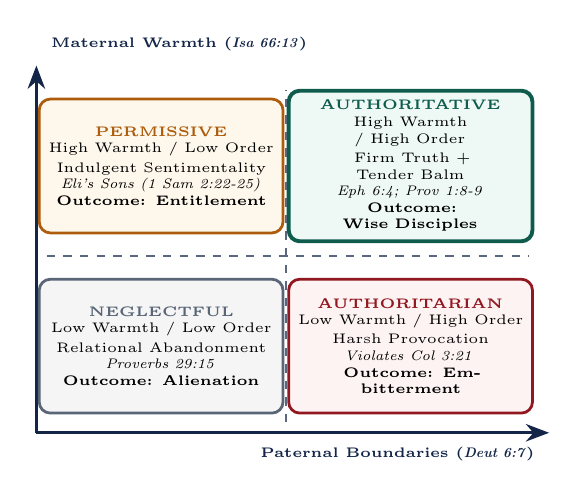
\begin{tikzpicture}[scale=0.88, >=Stealth,
    qbox/.style={rectangle, rounded corners=4pt, line width=1.0pt, text width=2.85cm, minimum height=1.7cm, align=center, font=\tiny, inner sep=3.5pt}
]
  % Axes
  \draw[->, line width=1.2pt, covenantblue] (0,0) -- (7.4,0) node[below left=2pt, font=\tiny\bfseries] {Paternal Boundaries (\textit{Deut 6:7})};
  \draw[->, line width=1.2pt, covenantblue] (0,0) -- (0,5.3) node[above right=2pt, font=\tiny\bfseries] {Maternal Warmth (\textit{Isa 66:13})};

  % Quadrant 1: Permissive (Top Left)
  \node[qbox, draw=filialamber, fill=filialamberfill] at (1.8, 3.85) {
    \textbf{\textcolor{filialamber}{PERMISSIVE}}\\
    High Warmth / Low Order\\[1pt]
    Indulgent Sentimentality\\
    \textit{Eli's Sons (1 Sam 2:22-25)}\\
    \textbf{Outcome: Entitlement}
  };

  % Quadrant 2: Christian Authoritative (Top Right)
  \node[qbox, draw=hearthteal, line width=1.4pt, fill=hearthtealfill] at (5.4, 3.85) {
    \textbf{\textcolor{hearthteal}{AUTHORITATIVE}}\\
    High Warmth / High Order\\[1pt]
    Firm Truth + Tender Balm\\
    \textit{Eph 6:4; Prov 1:8-9}\\
    \textbf{Outcome: Wise Disciples}
  };

  % Quadrant 3: Neglectful (Bottom Left)
  \node[qbox, draw=slateborder, fill=gray!8] at (1.8, 1.25) {
    \textbf{\textcolor{slateborder}{NEGLECTFUL}}\\
    Low Warmth / Low Order\\[1pt]
    Relational Abandonment\\
    \textit{Proverbs 29:15}\\
    \textbf{Outcome: Alienation}
  };

  % Quadrant 4: Authoritarian (Bottom Right)
  \node[qbox, draw=sacrificialred, fill=sacrificialredfill] at (5.4, 1.25) {
    \textbf{\textcolor{sacrificialred}{AUTHORITARIAN}}\\
    Low Warmth / High Order\\[1pt]
    Harsh Provocation\\
    \textit{Violates Col 3:21}\\
    \textbf{Outcome: Embitterment}
  };

  % Center Dividers cleanly in the gaps
  \draw[dashed, line width=0.9pt, covenantblue!70] (3.6, 0.15) -- (3.6, 4.95);
  \draw[dashed, line width=0.9pt, covenantblue!70] (0.15, 2.55) -- (7.1, 2.55);
\end{tikzpicture}
\caption{\textbf{The Christian Authoritative Parenting Matrix.} Optimal child formation synthesizes high paternal structure with high maternal responsiveness.}
\label{fig:parenting_matrix}
\end{figure}

\section{The Duties of Children Toward Parents}

\subsection{The Fourth Commandment: Honor and Reverence}
In the Decalogue, the Fourth Commandment bridges the love of God and the love of neighbor: ``Honor your father and your mother, that your days may be long in the land that the Lord your God is giving you'' (Exodus 20:12; Deuteronomy 5:16). St.~Paul notes this is the first commandment with a promise (Ephesians 6:2).

The Hebrew term for honor, \textit{kavod}, implies weightiness, treating parents with gravity and reverence. The opposite behavior, treating parents lightly or with contempt (\textit{qalal}), was a severe offense under Mosaic law (Exodus 21:17; Leviticus 20:9; Deuteronomy 27:16). In Catholic moral theology, St.~Thomas Aquinas classifies filial piety (\textit{pietas}) under the virtue of justice (\textit{Summa Theologiae} II-II, q. 101, a. 1) \cite{aquinas_summa}. Because parents are secondary principles of our being and governance after God, children owe them reverence, gratitude, and support.

\subsection{Scriptural Directives for Filial Conduct}
\begin{enumerate}
    \item \textbf{Prompt Obedience in Childhood}: ``Children, obey your parents in everything, for this pleases the Lord'' (Colossians 3:20; Ephesians 6:1). Disobedience to parents characterizes societal disintegration (Romans 1:30; 2 Timothy 3:2).
    \item \textbf{Receptive Listening to Instruction}: ``Hear, my son, your father's instruction, and forsake not your mother's teaching, for they are a graceful garland for your head and pendants for your neck'' (Proverbs 1:8-9).
    \item \textbf{Lifelong Material and Moral Care}: The Fourth Commandment extends across the entire lifespan. In 1 Timothy 5:4, adult children are commanded to ``make some return to their parents, for this is pleasing in the sight of God.'' Sirach 3:12-14 enjoins: ``My son, help your father in his old age, and do not grieve him as long as he lives; even if he lacks understanding, show forbearance.''
\end{enumerate}

\section{Game-Theoretic Proof of Covenantal Equilibrium}

Secular contractual marriage often deteriorates into a repeated Prisoner's Dilemma, where fear of exploitation incentivizes mutual defensiveness or defection. We model the Christian covenant as an extensive-form game between Husband ($H$) and Wife ($W$).

Let strategy sets be $\Sigma_i = \{\text{Sacrificial Love } (S), \text{Self-Serving Defection } (D)\}$. In a secular game, defection yields payoffs:
\begin{equation}
    u_i(D, S) = T = 5, \quad u_i(S, S) = R = 3
\end{equation}
\begin{equation}
    u_i(D, D) = P = 0, \quad u_i(S, D) = S_0 = -3
\end{equation}
Because $T > R > P > S_0$, mutual defection $(D,D)$ is the unique static Nash equilibrium.

In a Christian covenant, behavior is transformed by the presence of God as witness and enforcer. The utility function incorporates the divine sanction and eternal reward for each spouse $i \in \{H, W\}$:
\begin{equation}
    U_i(\sigma_H, \sigma_W) = u_i(\sigma_H, \sigma_W) + \gamma_i \mathbb{E}[V_C] - \theta_i \mathbb{I}(\sigma_i = D)
\end{equation}
where $\theta_i$ represents the spiritual cost of covenant violation, and $\gamma_i$ represents the sanctification valuation.

When $\theta_H > T - R$ and $\theta_W > T - R$, the payoff matrix satisfies $U_i(S, S) > U_i(D, S)$. Consequently, $(S,S)$, the strategy of kenotic male headship and respectful female honor, becomes the strictly dominant, subgame-perfect Nash equilibrium (Figure~\ref{fig:game_tree}). Covenantal marriage eliminates defection risk through shared submission to the sovereignty of Christ.

\begin{figure}[H]
\centering
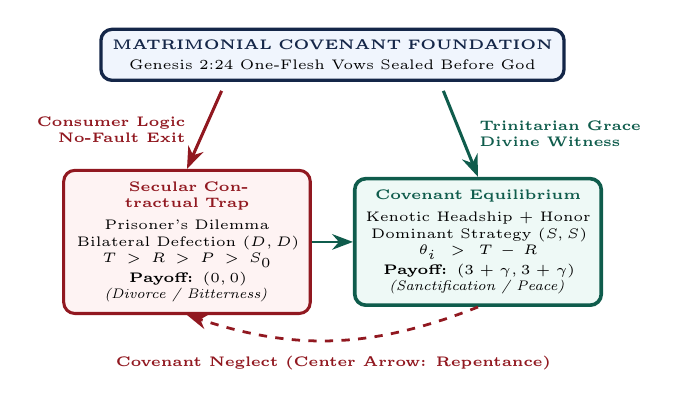
\begin{tikzpicture}[scale=0.88, >=Stealth,
    rootbox/.style={rectangle, rounded corners=4pt, draw=covenantblue, line width=1.2pt, fill=covenantbluefill, text width=5.6cm, align=center, font=\tiny, inner sep=4pt},
    secularbox/.style={rectangle, rounded corners=4pt, draw=sacrificialred, line width=1.1pt, fill=sacrificialredfill, text width=2.85cm, align=center, font=\tiny, inner sep=4pt},
    covbox/.style={rectangle, rounded corners=4pt, draw=hearthteal, line width=1.3pt, fill=hearthtealfill, text width=2.85cm, align=center, font=\tiny, inner sep=4pt}
]
  % Root node
  \node[rootbox] (root) at (0, 3.8) {
    \textbf{\textcolor{covenantblue}{MATRIMONIAL COVENANT FOUNDATION}}\\[1pt]
    Genesis 2:24 One-Flesh Vows Sealed Before God
  };

  % Secular Trap (Left)
  \node[secularbox] (secular) at (-2.1, 1.1) {
    \textbf{\textcolor{sacrificialred}{Secular Contractual Trap}}\\[2pt]
    Prisoner's Dilemma\\
    Bilateral Defection $(D,D)$\\
    $T > R > P > S_0$\\[1pt]
    \textbf{Payoff: $(0, 0)$}\\
    \textit{(Divorce / Bitterness)}
  };

  % Covenant Equilibrium (Right)
  \node[covbox] (covenant) at (2.1, 1.1) {
    \textbf{\textcolor{hearthteal}{Covenant Equilibrium}}\\[2pt]
    Kenotic Headship + Honor\\
    Dominant Strategy $(S,S)$\\
    $\theta_i > T - R$\\[1pt]
    \textbf{Payoff: $(3+\gamma, 3+\gamma)$}\\
    \textit{(Sanctification / Peace)}
  };

  % Branching Arrows from Root
  \draw[->, line width=1.1pt, sacrificialred] (-1.6, 3.28) --
    node[left=3pt, font=\tiny\bfseries, text=sacrificialred, align=right] {Consumer Logic\\No-Fault Exit} (secular.north);

  \draw[->, line width=1.1pt, hearthteal] (1.6, 3.28) --
    node[right=3pt, font=\tiny\bfseries, text=hearthteal, align=left] {Trinitarian Grace\\Divine Witness} (covenant.north);

  % Top Restitution Arrow in center gap
  \draw[->, line width=1.0pt, hearthteal] (secular.east) -- (covenant.west);

  % Bottom Decay Arc below boxes
  \draw[->, line width=1.0pt, dashed, sacrificialred] (covenant.south) to[bend left=20]
    node[below=2pt, font=\tiny\bfseries, text=sacrificialred] {Covenant Neglect (Center Arrow: Repentance)} (secular.south);
\end{tikzpicture}
\caption{\textbf{Marital State Transitions and Game Equilibrium.} The transcendent presence of God shifts the social dynamic from contractual defection to permanent cooperative sanctification.}
\label{fig:game_tree}
\end{figure}

\section{Conclusion}
The philosophy of Christian marriage and the covenant family offers an unyielding architecture of relational flourishing amidst cultural disintegration. Grounded in the creation order of Genesis, elevated by the sacramental mystery of Christ and the Church, and ordered by differentiated hierarchical offices, the Christian household functions as an impenetrable fortress of virtue. In this domestic church, the husband leads by surrendering his life in sacrificial love, the wife reigns as the executive heart of the home in royal honor, and the children grow in reverent obedience under authoritative instruction, transmitting the light of faith across generations.

\section*{Declarations}

\subsection*{Data and code availability}
All game-theoretic payoffs, mathematical derivations, and structural modeling scripts generated in support of this research are archived in the repository and are reproducible in standard Python numerical environments.

\subsection*{Use of generative AI}
During the preparation of this manuscript, the author utilized generative artificial intelligence models, specifically Claude, GPT-OSS, and Gemini, to assist in literature indexing, Latin cross-referencing, and structural validation. The author verified every citation, derived all mathematical models, authored all philosophical discourse, and assumes full responsibility for the manuscript.

\subsection*{Authorship, funding and competing interests}
The author declares that this research received no commercial or institutional grant funding. The author reports no competing financial or non-financial conflicts of interest.

\begin{thebibliography}{99}
\bibitem{aquinas_summa} Aquinas, T. (1274). \textit{Summa Theologiae}, Supplementum, Questions 41--68 (On the Sacrament of Matrimony); Second Part of the Second Part, Question 26 (On the Order of Charity); Question 101 (On Piety). Translated by Fathers of the English Dominican Province, Benziger Brothers, 1920. \url{https://www.newadvent.org/summa/5049.htm}.
\bibitem{augustine_bono} Augustine of Hippo. (401). \textit{De Bono Coniugali} (On the Good of Marriage) and \textit{De Nuptiis et Concupiscentia} (On Marriage and Concupiscence). Translated by C. L. Cornish, Nicene and Post-Nicene Fathers, First Series, Vol. 3, edited by P. Schaff, Christian Literature Publishing Co., 1887. \url{https://www.newadvent.org/fathers/1309.htm}.
\bibitem{bavinck} Bavinck, H. (1908). \textit{The Christian Family}. Translated by N. D. Kloosterman, Christian's Library Press, 2012.
\bibitem{baxter} Baxter, R. (1673). \textit{A Christian Directory: A Sum of Practical Theology and Cases of Conscience}, Part II: Christian Economics (Family Duties). Soli Deo Gloria Publications, 1997. \url{https://www.gutenberg.org/files/43800/43800-h/43800-h.htm}.
\bibitem{chrysostom_eph} Chrysostom, J. (c. 392). \textit{Homilies on the Epistle of St. Paul to the Ephesians}, Homily XX and Homily XXI. Translated by G. Grossmann, Nicene and Post-Nicene Fathers, First Series, Vol. 13, edited by P. Schaff, Christian Literature Publishing Co., 1889. \url{https://www.newadvent.org/fathers/230120.htm}.
\bibitem{chrysostom_marriage} Chrysostom, J. (c. 390). \textit{On Marriage and Family Life}. Translated by C. P. Roth and D. Anderson, St. Vladimir's Seminary Press, 1986.
\bibitem{calvin_inst} Calvin, J. (1559). \textit{Institutes of the Christian Religion}. Edited by J. T. McNeill, translated by F. L. Battles, Westminster John Knox Press, 1960.
\bibitem{edwards} Edwards, J. (1751). \textit{The Nature of True Virtue}. Edited by P. Ramsey, Yale University Press, 1989.
\bibitem{henry} Henry, M. (1708). \textit{An Exposition of the Old and New Testament}, Vol. 1: Genesis to Deuteronomy. Commentary on Genesis 2:21--25. \url{https://www.biblegateway.com/resources/matthew-henry/Gen.2.21-Gen.2.25}.
\bibitem{leo_arcanum} Leo XIII. (1880). \textit{Arcanum Divinae Sapientiae} (Encyclical on Christian Marriage). Vatican Polyglot Press. \url{https://www.vatican.va/content/leo-xiii/en/encyclicals/documents/hf_l-xiii_enc_10021880_arcanum.html}.
\bibitem{luther_estate} Luther, M. (1522). \textit{The Estate of Marriage} (\textit{Vom ehelichen Leben}). In \textit{Luther's Works}, Vol. 45: The Christian in Society II, edited by W. I. Brandt, Fortress Press, 1962.
\bibitem{perkins} Perkins, W. (1609). \textit{Christian Oeconomie: Or, A Short Survey of the Right Manner of Erecting and Ordering a Familie, According to the Scriptures}. Translated by T. Pickering, Felix Kingston, London. \url{https://archive.org/details/christian_oeconomie_2312_librivox}.
\bibitem{piper} Piper, J., \& Grudem, W. (Eds.). (1991). \textit{Recovering Biblical Manhood and Womanhood: A Response to Evangelical Feminism}. Crossway Books.
\bibitem{pius_casti} Pius XI. (1930). \textit{Casti Connubii} (Encyclical on Christian Marriage in Contrast to Present Conditions). Vatican Polyglot Press. \url{https://www.vatican.va/content/pius-xi/en/encyclicals/documents/hf_p-xi_enc_19301231_casti-connubii.html}.
\end{thebibliography}

\end{document}
